در این پوشه رابط تعامل کاربر با سیستم انجام می‌شود.

\begin{figure}[H]
	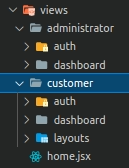
\includegraphics[width=.3\textwidth]{Folders-Files/views.png}
	\centering
	\caption{ساختار پوشه نما}
	\label{fig:folder-views}
\end{figure}


\paragraph{پوشه administrator}
در این پوشه به قالب مدیریت پرداخته شده است.

\subparagraph{پوشه auth}
در این پوشه به قالب احرازهویت مدیریت پرداخته شده است.

\subparagraph{پوشه dashboard}
در این پوشه به قالب داشبورد مدیریت پرداخته شده است.

\subparagraph{پوشه component}
در این پوشه به قالب تکرارشونده مانند منوها، هدر، فوتر و ... پرداخته شده است.


\paragraph{فایل customer}
در این پوشه به قالب کاربر پرداخته شده است.

\subparagraph{پوشه auth}
در این پوشه به قالب احرازهویت کاربر پرداخته شده است.

\subparagraph{فایل login}
در این فایل به قالب ورود کاربر پرداخته شده است.

\subparagraph{فایل signup}
در این فایل به قالب ثبت‌نام کاربر پرداخته شده است.

\subparagraph{پوشه dashboard}
در این پوشه به قالب داشبوردهای کارفرما و فریلنسر پرداخته شده است.

\subparagraph{پوشه component}
در این پوشه به قالب تکرارشونده مانند منوها، هدر، فوتر و ... پرداخته شده است.